\documentclass[10pt,twocolumn]{article}

\usepackage[margin=1in]{geometry}
\usepackage{amsmath,amssymb}
\usepackage{booktabs}
\usepackage{graphicx}
\usepackage{pgfplots}
\pgfplotsset{compat=1.18}
\usepackage{tikz}
\usetikzlibrary{arrows.meta,positioning,shapes.geometric,fit,calc}
\usepackage{hyperref}
\usepackage[numbers]{natbib}
\usepackage{xcolor}
\usepackage{enumitem}
\usepackage[expansion=false]{microtype}
\usepackage{caption}
\usepackage{multirow}
\usepackage{siunitx}
\usepackage{pifont}

\setlength{\columnsep}{0.25in}
\emergencystretch=1em

% Consistent color palette
\definecolor{cfresh}{HTML}{2196F3}
\definecolor{cfull}{HTML}{4CAF50}
\definecolor{ctargeted}{HTML}{FF9800}
\definecolor{cbaseline}{HTML}{9E9E9E}
\definecolor{cthorne}{HTML}{E91E63}
\definecolor{cchain1}{HTML}{90CAF9}
\definecolor{cchain2}{HTML}{A5D6A7}
\definecolor{cchain3}{HTML}{FFCC80}
\definecolor{cchain4}{HTML}{CE93D8}

\title{Coordinated Goal Evolution Restores Structural Quality\\in Deterministic Narrative Simulation Chains}
\author{
  Jack Chaudier Gaffney\\
  \texttt{jackchaudier@gmail.com}
}
\date{}

\begin{document}
\maketitle

% ============================================================
% ABSTRACT
% ============================================================
\begin{abstract}
Multi-agent narrative simulations that carry persistent world state across episodes face a structural degradation problem: as agents' fixed goals become misaligned with the evolved story world, arc quality declines. We present \textsc{NarrativeField}, a deterministic simulation-extraction pipeline for multi-protagonist stories, and identify \emph{information depletion}---the exhaustion of secrets, unresolved tensions, and belief asymmetries---as the root cause. A controlled perturbation experiment provides evidence that, within our pipeline, belief-state content causally affects extracted arc structure, with structurally central propositions producing order-of-magnitude larger quality effects than peripheral controls. Coordinated goal evolution across all six agents closes 89\% of the quality gap between degraded and fresh simulations, revealing a collective threshold effect: single-agent evolution \emph{degrades} quality, while coordinated evolution restores it. All experiments run deterministically at zero LLM cost with full reproducibility from fixed random seeds.
\end{abstract}

% ============================================================
% 1. INTRODUCTION
% ============================================================
\section{Introduction}
\label{sec:intro}

Emergent narrative systems promise stories that arise from simulated character interactions rather than pre-authored plot structures~\cite{cavazza2002character,ryan2015open}. Unlike plan-based approaches that search over action sequences toward a desired ending~\cite{riedl2010narrative,young2013plans}, simulation-first systems let narrative structure emerge from agent decision-making under social pressure. This approach has produced compelling results in single-episode settings~\cite{mateas2003facade,park2023generative}, but a fundamental challenge arises when simulations must produce \emph{sequential} stories sharing persistent world state.

We identify and formalize a \emph{chain degradation} problem: when world canon---accumulated beliefs, relationship states, and resolved secrets---carries forward between episodes, agents with fixed goal vectors find themselves in an information-saturated environment where the dramatic fuel that powered earlier stories has been consumed. Secrets are known, alliances are settled, and the decision engine's utility landscape flattens. The result is measurable: across four independent chain orderings of five-story sequences, mean arc quality scores show an overall downward trend by position, from $0.696$ at position~0 to $0.637$ at position~4 (Figure~\ref{fig:chain_trend}).

This paper makes four contributions:
\begin{enumerate}[nosep]
\item We demonstrate \emph{chain degradation} as a systematic, ordering-robust phenomenon in multi-episode narrative simulation, reducing the plausibility that the observed decline is a seed-order artifact.
\item We introduce a \emph{belief-state perturbation} experiment providing evidence that, within our deterministic pipeline, narrative structure is causally sensitive to belief propositions, with structurally central claims producing order-of-magnitude larger quality effects than peripheral controls.
\item We present \emph{coordinated goal evolution} as a mechanism for restoring narrative quality in information-depleted environments, closing 89\% of the degradation gap.
\item We show that goal evolution exhibits a \emph{collective threshold}: single-agent evolution degrades quality ($-0.027$), while coordinated six-agent evolution improves it ($+0.047$), supporting the hypothesis that narrative quality in our system is strongly shaped by the agent interaction topology.
\end{enumerate}

All experiments are fully deterministic and reproducible from fixed random seeds.\footnote{Chain seeds: 42, 51, 7, 13, 29 (four orderings). Evolution experiment: seed~7. Configuration files and experiment scripts available upon request.} The simulation, metrics, and arc extraction pipeline runs without LLM calls, at \$0.00 compute cost per experimental condition via skip-narration mode.


% ============================================================
% 2. RELATED WORK
% ============================================================
\section{Related Work}
\label{sec:related}

\paragraph{Multi-agent narrative simulation.}
Character-driven narrative has a long history from \textsc{Tale-Spin}~\cite{meehan1977tale} through \textsc{Fa\c{c}ade}~\cite{mateas2003facade} and \textsc{Thespian}~\cite{si2005thespian}. Recent work on generative agents demonstrated that LLM-backed characters produce emergent social behavior in open-ended sandbox environments~\cite{park2023generative}. Our system differs in using deterministic utility-based agents with explicit goal vectors rather than LLM inference for decision-making, enabling reproducible experiments and controlled causal analysis within the pipeline.

\paragraph{Narrative planning.}
Plan-based approaches search action spaces for sequences satisfying narrative goals~\cite{riedl2010narrative,young2013plans}. \textsc{C2PO} introduced causal commonsense ordering constraints~\cite{ammanabrolu2021c2po}; neural planners use learned models to propose plot outlines~\cite{ye2022neural}. These systems optimize for coherent plot structure but typically lack agent autonomy. Goal-Oriented Action Planning (GOAP)~\cite{orkin2006goap} bridges planning and agent autonomy but focuses on single-agent tactical behavior. Our approach inverts the pipeline: simulate first, extract structure post-hoc.

\paragraph{Story sifting and extraction.}
Story sifting~\cite{garbe2019storysifting} retrieves narrative patterns from simulation logs. \textsc{Winnow}~\cite{kreminski2020winnow} provides a domain-specific language for incremental sifting queries. Our Rashomon extraction generalizes sifting by extracting complete per-protagonist arc structures with grammar validation and composite scoring, rather than pattern-matching individual story moments.

\paragraph{Long-form narrative coherence.}
Maintaining coherence across extended narratives is recognized as a key challenge~\cite{akoury2023framework}. Multi-agent collaborative generation with specialized roles has shown promise for document-length text~\cite{pmlr2025agents}. BDI architectures for interactive narrative~\cite{wadsley2013bdi} provide a related formalism for persistent agent state. Our work specifically addresses the under-explored problem of \emph{sequential} story coherence when world state persists across episodes.


% ============================================================
% 3. SYSTEM DESCRIPTION
% ============================================================
\section{System Description}
\label{sec:system}

\textsc{NarrativeField} is a four-stage pipeline (Figure~\ref{fig:architecture}): simulation, metrics computation, arc extraction, and optional prose rendering. Steps~1--3 are fully deterministic; step~4 uses an LLM for prose generation but is not required for evaluation. All results in this paper use only the deterministic stages.

\begin{figure*}[t]
\centering
\resizebox{\textwidth}{!}{%
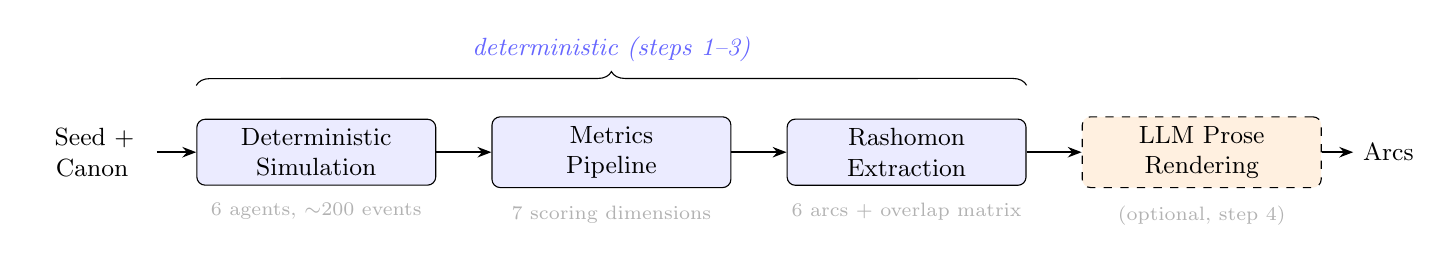
\begin{tikzpicture}[
  node distance=0.7cm,
  box/.style={draw, rounded corners=3pt, minimum height=0.7cm, text width=2.8cm, align=center, font=\small},
  detbox/.style={box, fill=blue!8},
  llmbox/.style={box, fill=orange!12, dashed},
  arr/.style={-{Stealth[length=5pt]}, thick},
  sublabel/.style={font=\scriptsize, text=gray!60},
]
\node[detbox] (sim) {Deterministic\\Simulation};
\node[detbox, right=of sim] (met) {Metrics\\Pipeline};
\node[detbox, right=of met] (arc) {Rashomon\\Extraction};
\node[sublabel, below=0.1cm of sim] {6 agents, ${\sim}200$ events};
\node[sublabel, below=0.1cm of met] {7 scoring dimensions};
\node[sublabel, below=0.1cm of arc] {6 arcs + overlap matrix};

\node[llmbox, right=of arc] (llm) {LLM Prose\\Rendering};
\node[sublabel, below=0.1cm of llm] {(optional, step 4)};

\node[font=\small, text width=1.4cm, align=center, left=0.5cm of sim] (inp) {Seed +\\Canon};
\node[font=\small, right=0.4cm of llm] (out) {Arcs};

\draw[arr] (inp) -- (sim);
\draw[arr] (sim) -- (met);
\draw[arr] (met) -- (arc);
\draw[arr] (arc) -- (llm);
\draw[arr] (llm) -- (out);

% Brace for deterministic stages
\draw[decorate, decoration={brace, amplitude=5pt, raise=12pt}] (sim.north west) -- (arc.north east)
  node[midway, above=17pt, font=\small\itshape, text=blue!60] {deterministic (steps 1--3)};
\end{tikzpicture}
}
\caption{System pipeline. Steps~1--3 are fully deterministic and produce all metrics reported in this paper. Step~4 (LLM prose rendering) is optional and was disabled for all experiments.}
\label{fig:architecture}
\end{figure*}

\subsection{Simulation Engine}
\label{sec:simulation}

The simulation operates on discrete ticks with an event queue for simultaneous action resolution. Six agents---Thorne, Elena, Marcus, Lydia, Diana, and Victor---interact across five locations (dining table, kitchen, balcony, foyer, bathroom) with privacy, adjacency, and overhearing rules.

\paragraph{Agent state.} Each agent maintains a \texttt{GoalVector} with seven utility dimensions: \emph{safety}, \emph{status}, \emph{closeness} (a per-target dictionary), \emph{secrecy}, \emph{truth\_seeking}, \emph{autonomy}, and \emph{loyalty}. Relationships are modeled as per-target triples of \emph{trust}, \emph{affection}, and \emph{obligation} on $[-1, 1]$. Each agent holds categorical beliefs over propositions: \texttt{unknown}, \texttt{suspects}, \texttt{believes\_true}, or \texttt{believes\_false}.

\paragraph{Decision engine.} At each tick, the engine scores candidate actions via:
\begin{align}
\label{eq:utility}
u(a) ={} & u_{\text{base}}(a) + b_{\text{flaw}}(a) + m_{\text{pace}}(a) \notag \\
         & + m_{\text{rel}}(a) - p_{\text{rec}}(a) + \epsilon
\end{align}
where $u_{\text{base}}$ evaluates goal-weighted action effects across all seven dimensions, $b_{\text{flaw}}$ applies character flaw biases, $m_{\text{pace}}$ enforces pacing physics (dramatic budget, stress, composure, hysteresis), $m_{\text{rel}}$ modifies for relationship state, $p_{\text{rec}}$ penalizes recently taken actions, and $\epsilon$ is drawn from a seeded pseudorandom generator. The agent selects $a^* = \arg\max_a u(a)$; the seeded noise term $\epsilon$ serves as a deterministic tiebreaker, ensuring identical action sequences given identical seeds. Additionally, \textsc{social\_move} actions receive a fixed $-0.10$ penalty to discourage unproductive movement, and \textsc{internal} actions are capped at $u \leq 0.45$ to prevent inaction from dominating dramatic choices.

\paragraph{Event types.} The simulation produces ten event types: \textsc{chat}, \textsc{observe}, \textsc{social\_move}, \textsc{reveal}, \textsc{conflict}, \textsc{internal}, \textsc{physical}, \textsc{confide}, \textsc{lie}, and \textsc{catastrophe}. Each run generates approximately 200 events over 30 simulation ticks.

\paragraph{Wounds.} A \emph{wound} is a persistent conflict dyad: a pair of agents who engage in repeated \textsc{conflict} events at the same location during a simulation. The \emph{wound topology} is the set of active wounds across a run; we use it to track how the social conflict graph restructures under different experimental conditions (Section~\ref{sec:evolution}).

\paragraph{World canon.} A \texttt{WorldCanon} object accumulates persistent state between sequential stories: per-location tension residue, agent belief states with confidence scores, and committed texture facts. The engine supports configurable exponential decay between episodes (tension at rate $\alpha_t$ and belief confidence at rate $\alpha_b$, with beliefs reverting to \texttt{unknown} below confidence~$0.1$). However, all chain experiments reported in this paper use no-decay settings ($\alpha_t = \alpha_b = 1.0$); a separate decay experiment found zero structural effect (Section~\ref{sec:failed_interventions}).

\subsection{Metrics Pipeline}
\label{sec:metrics}

Arc quality is measured by a composite score $Q$ aggregating seven normalized dimensions ($M_i \in [0,1]$):
\begin{align}
\label{eq:composite}
Q ={} & 0.20\,M_{\text{var}} + 0.15\,M_{\text{peak}} + 0.15\,M_{\text{shape}} \notag \\
      & + 0.15\,M_{\text{sig}} + 0.15\,M_{\text{theme}} \notag \\
      & + 0.10\,M_{\text{irony}} + 0.10\,M_{\text{prot}}
\end{align}
where $M_{\text{var}}$ is tension variance (normalized by a fixed constant of $0.013$), $M_{\text{peak}}$ is peak tension magnitude, $M_{\text{shape}}$ rewards rising-then-falling tension profiles, $M_{\text{sig}}$ measures the impact of events at turning points, $M_{\text{theme}}$ evaluates thematic thread coherence across events, $M_{\text{irony}}$ rewards dramatic irony (events where audience knowledge exceeds participant knowledge), and $M_{\text{prot}}$ measures how central the focal agent is to their own arc. All $M_i$ are normalized to $[0,1]$ using fixed constants defined in the scoring implementation; $M_{\text{var}}$ uses a normalization constant of $0.013$ derived from population-level tension statistics. Tension-related dimensions ($M_{\text{var}} + M_{\text{peak}} + M_{\text{shape}}$) collectively account for 50\% of the composite; the remaining 50\% comes from structural, thematic, and dramatic irony dimensions. Weights were fixed across all experimental conditions; no per-condition tuning was performed. All metrics are computed deterministically from event logs.

\subsection{Rashomon Extraction}
\label{sec:rashomon}

Following the principle that a single sequence of events contains multiple valid narratives depending on whose perspective is centered~\cite{kurosawa1950rashomon}, we extract one arc per agent per simulation. Each arc selects up to 20 events and validates against a beat grammar with the following constraints:

\begin{itemize}[nosep]
\item At least one \textsc{setup}, one \textsc{consequence}, and exactly one \textsc{turning\_point} beat.
\item At least one development beat (\textsc{complication} or \textsc{escalation}; these are interchangeable within the development phase).
\item Monotonic phase progression: setup~$\to$ development~$\to$ crisis~$\to$ resolution (no phase reversals).
\item Beat count between 4 and 20 (inclusive).
\item Protagonist appears in $\geq$60\% of arc events.
\item Causal continuity: each event shares a causal link or participant overlap with its predecessor.
\item Temporal span $\geq$10 sim-minutes and $\geq$15\% of total simulation time.
\end{itemize}

A \texttt{RashomonSet} contains all six per-protagonist arcs, their composite scores, and a Jaccard overlap matrix quantifying narrative divergence. Population-level validation across 50 seeds yields 294/300 valid arcs (98\%) with 44/50 seeds producing six valid arcs (88\%).


% ============================================================
% 4. CHAIN DEGRADATION PROBLEM
% ============================================================
\section{The Chain Degradation Problem}
\label{sec:degradation}

\subsection{Observation}
\label{sec:chain_obs}

We run five-story chains ($A \to B \to C \to D \to E$) where each story's simulation loads the accumulated canon from all prior stories. To control for seed-specific effects, we run four independent orderings of the same five seeds (42, 51, 7, 13, 29) and average scores by chain position. Table~\ref{tab:chain_position} and Figure~\ref{fig:chain_trend} show the results.

\begin{table}[t]
\centering
\caption{Mean arc score by chain position, averaged across four independent seed orderings. Overall downward trend with local variation at position~3.}
\label{tab:chain_position}
\begin{tabular}{lcc}
\toprule
\textbf{Position} & \textbf{Mean Score} & \textbf{$\Delta$ from Pos.~0} \\
\midrule
0 (first story) & 0.696 & --- \\
1               & 0.679 & $-0.017$ \\
2               & 0.644 & $-0.052$ \\
3               & 0.650 & $-0.046$ \\
4 (fifth story) & 0.637 & $-0.059$ \\
\bottomrule
\end{tabular}
\end{table}

\begin{figure}[t]
\centering
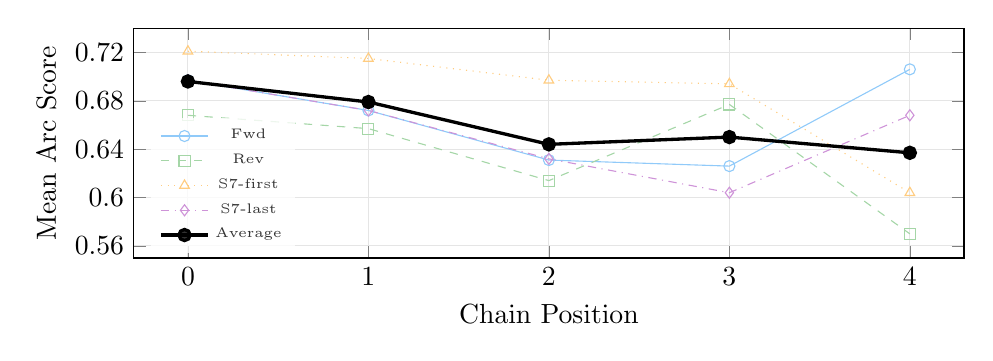
\begin{tikzpicture}
\begin{axis}[
  width=\columnwidth,
  height=4.5cm,
  xlabel={Chain Position},
  ylabel={Mean Arc Score},
  xmin=-0.3, xmax=4.3,
  ymin=0.55, ymax=0.74,
  xtick={0,1,2,3,4},
  xticklabels={0,1,2,3,4},
  ytick={0.56,0.60,0.64,0.68,0.72},
  grid=major,
  grid style={gray!20},
  legend style={at={(0.02,0.02)}, anchor=south west, font=\tiny, draw=none, fill=white, fill opacity=0.8},
  every axis plot/.append style={mark size=2pt},
]
% Individual orderings (faint, distinct dash patterns for grayscale)
\addplot[cchain1, thin, solid, mark=o, mark options={solid}]
  coordinates {(0,0.697)(1,0.672)(2,0.631)(3,0.626)(4,0.706)};
\addplot[cchain2, thin, dashed, mark=square, mark options={solid}]
  coordinates {(0,0.668)(1,0.657)(2,0.614)(3,0.677)(4,0.570)};
\addplot[cchain3, thin, dotted, mark=triangle, mark options={solid}]
  coordinates {(0,0.721)(1,0.715)(2,0.697)(3,0.694)(4,0.604)};
\addplot[cchain4, thin, dashdotted, mark=diamond, mark options={solid}]
  coordinates {(0,0.697)(1,0.672)(2,0.632)(3,0.604)(4,0.668)};
% Position average (bold)
\addplot[black, very thick, mark=*, mark options={solid, fill=black}]
  coordinates {(0,0.696)(1,0.679)(2,0.644)(3,0.650)(4,0.637)};
\legend{Fwd, Rev, S7-first, S7-last, Average}
\end{axis}
\end{tikzpicture}
\caption{Mean arc score by chain position. Bold black line: position-averaged means across four seed orderings. Thin lines: individual orderings with distinct dash patterns for grayscale readability. Three of four orderings show negative first-to-last slope; one (Forward, solid) exhibits a U-shaped recovery at position~4 that does not replicate under averaging.}
\label{fig:chain_trend}
\end{figure}

Three of four orderings show negative first-to-last slope; one ordering (seeds 42, 51, 7, 13, 29) exhibits a U-shaped recovery at position~4 ($0.697 \to 0.672 \to 0.631 \to 0.626 \to 0.706$) that did not replicate under seed-order controls, substantially reducing the likelihood that the observed degradation is only a seed-order artifact. The position-averaged means show a clear overall decline of $-0.059$ from position~0 to position~4 despite a local rebound at position~3.

For context, across the 50-seed Rashomon sweep at depth~0, per-seed mean arc scores have standard deviation $\sigma = 0.037$ (294 valid arcs, mean $0.674$). The full-evolution lift of $+0.047$ reported in Section~\ref{sec:evolution} corresponds to approximately $1.3\sigma$ of this baseline population distribution, providing a rough effect-size calibration despite the single-seed limitation of the evolution experiment.


\subsection{Failed Interventions}
\label{sec:failed_interventions}

Three prior interventions targeting different canon fields all produced zero measurable structural effect on arc quality, converging on the diagnosis that the decision engine consumes a narrower state interface than the full canon schema suggests.

\paragraph{Texture accumulation.} Over a five-story chain, 69 narrator-invented texture facts (wine labels, physical gestures, room descriptions) accumulated in the canon. These feed into subsequent narration prompts but have zero structural effect: skip-narration runs produce identical metrics with or without texture. Texture and simulation structure are orthogonal channels.

\paragraph{Belief confidence decay.} A float-valued confidence score was added to each belief, decayed by $0.85\times$ between episodes. This produced zero structural effect because the simulation's decision engine reads categorical \texttt{claim\_states} (string enums), not confidence floats. Decaying a field that no decision path reads changes nothing.

\paragraph{Tension residue decay.} Per-location tension residue was decayed by $0.60\times$ between episodes. Zero structural effect: within-run tension decay ($0.97\times$ per tick) dominates any starting residue, making inter-episode tension memory irrelevant to action selection.

These null results motivated the perturbation experiment (Section~\ref{sec:perturbation}), which directly probes which state fields the decision engine is actually sensitive to.


\subsection{Diagnosis}
\label{sec:diagnosis}

\begin{table}[t]
\centering
\caption{Belief states after Story~B (seed~7). Four of seven claims are universally \texttt{believes\_true} (BT), leaving only one structurally mixed claim. U\,=\,unknown, S\,=\,suspects, BF\,=\,believes\_false.}
\label{tab:canon_state}
\begin{tabular}{@{}lcccccc@{}}
\toprule
\textbf{Claim} & \textbf{Di} & \textbf{El} & \textbf{Ly} & \textbf{Ma} & \textbf{Th} & \textbf{Vi} \\
\midrule
affair        & BT & BT & BT & BT & BT & BT \\
diana\_debt    & BT & BT & BT & BT & BT & BT \\
lydia\_knows   & BT & BT & BT & BT & BT & BT \\
victor\_inv    & BT & BT & BT & BT & BT & BT \\
\midrule
embezzle      & U  & U  & S  & BT & U  & BF \\
guild\_press   & U  & U  & U  & U  & U  & U  \\
thorne\_health & U  & U  & U  & U  & U  & U  \\
\bottomrule
\end{tabular}
\end{table}

The degradation mechanism is \emph{information depletion}. Table~\ref{tab:canon_state} shows the concrete belief state after two episodes: four of seven claims are universally \texttt{believes\_true}---every agent knows every major secret. Only one claim (\texttt{embezzle}) retains meaningful disagreement. When agents carry forward this saturated knowledge, the space of dramatically productive actions shrinks: there is nothing to reveal, no secret worth protecting, and alliances are settled. Fixed goals in this changed information landscape produce \emph{goal--world misalignment}: agents optimize for objectives (e.g., Elena maintaining affair secrecy) that are no longer achievable or meaningful given what is universally known.


% ============================================================
% 5. EXPERIMENT 1: BELIEF STATE PERTURBATION
% ============================================================
\section{Experiment 1: Belief-State Perturbation}
\label{sec:perturbation}

\subsection{Method}

To test whether agent belief states causally affect narrative structure within our deterministic pipeline, we design a controlled perturbation experiment. Starting from the post-Story-B world state (seed~7), we introduce two single-belief mutations and measure their downstream impact on Story~C.

\paragraph{Primary mutation.} The selection script ranks mutable beliefs by three criteria: (1)~whether the claim involves a secret (thematic centrality to the scenario's primary conflicts), (2)~belief diversity across agents (number of distinct belief states, favoring claims with active disagreement), and (3)~agent importance (protagonist weighting). The intended primary target was Thorne's belief about \texttt{secret\_affair\_01}---the most thematically potent claim---but after two chain steps this belief is already \texttt{believes\_true} (Table~\ref{tab:canon_state}), making it immutable. The fallback selected Thorne$\,\times\,$\texttt{secret\_embezzle\_01} as the highest-ranked remaining candidate: the only secret with active belief disagreement (three \texttt{unknown}, one \texttt{suspects}, one \texttt{believes\_true}, one \texttt{believes\_false}). Thorne's belief was mutated from \texttt{unknown} to \texttt{suspects}. That the most potent candidate was already spent is itself evidence of information depletion.

\paragraph{Control mutation.} Diana's belief about \texttt{claim\_guild\_pressure}, a peripheral non-secret proposition with universal \texttt{unknown} status, mutated from \texttt{unknown} to \texttt{suspects}. Control selection avoids central tokens and prefers claims with low belief diversity.

\paragraph{Instrumentation.} A \texttt{TracedBeliefs} wrapper intercepts all belief-state reads during Story~C simulation, recording agent, claim, value, and access method for every read operation.

\subsection{Results}

\begin{table}[t]
\centering
\caption{Perturbation experiment results. Primary mutation to a structurally central belief produces ${\sim}16\times$ the quality impact of the peripheral control (exact ratio $15.8$ from unrounded values), with complete event-level divergence.}
\label{tab:perturbation}
\begin{tabular}{lcc}
\toprule
\textbf{Metric} & \textbf{Primary} & \textbf{Control} \\
\midrule
Mean score $\Delta$ & $-0.040$ & $-0.0025$ \\
First divergence tick & 0 & None \\
Event sequences identical & No & Yes \\
Wound topology changes & +2, $-$1 & None \\
Valid arcs & 6/6 & 6/6 \\
\bottomrule
\end{tabular}
\end{table}

Table~\ref{tab:perturbation} summarizes the results. The primary mutation produces a mean score delta of $-0.040$ (baseline $0.668 \to 0.628$), while the control mutation produces $-0.0025$ ($0.668 \to 0.666$). Event traces diverge at tick~0 for the primary mutation---the very first decision cycle reads the mutated belief and produces a different action---while the control mutation generates an \emph{identical} event sequence to baseline.

\paragraph{Belief trace analysis.} The instrumented run recorded 13{,}895 total belief reads across 42 unique agent-claim fields. The most-read field was Diana$\,\times\,$\texttt{secret\_affair\_01} with 913 reads, confirming that even fully-resolved propositions continue to dominate the decision engine's information consumption. The \texttt{secret\_embezzle\_01} claim appeared in the top-25 most-read fields for three agents (Elena: 321 reads, Diana: 319, Marcus: 279), consistent with its structural centrality as the sole asymmetric secret.

\paragraph{Wound topology shift.} The primary mutation caused two new conflict patterns to emerge (Diana--Thorne and Marcus--Thorne at the dining table) and one to disappear (Diana--Victor), restructuring the social conflict graph. The control mutation left the wound topology unchanged.

\subsection{Analysis}

These results provide evidence for two claims within our deterministic pipeline. First, narrative structure is \emph{causally sensitive} to belief-state content: changing a single categorical belief from \texttt{unknown} to \texttt{suspects} produces measurable structural consequences. Second, this sensitivity is \emph{specific to structurally central propositions}: peripheral beliefs can be mutated without observable effect, providing a natural control. The ${\sim}16\times$ effect size ratio ($-0.040$ vs.\ $-0.0025$) and the all-or-nothing divergence pattern (tick~0 vs.\ identical) suggest a sharp, threshold-like sensitivity pattern in this scenario, where central beliefs act as bifurcation points in the simulation's trajectory space.

The perturbation experiment confirmed that beliefs are causally active within our pipeline, but showed that individual belief mutations cannot rescue an information-depleted system---the problem is systemic. This motivates testing whether the root cause is not individual belief states but the \emph{goal structures} that interpret them.


% ============================================================
% 6. EXPERIMENT 2: GOAL EVOLUTION
% ============================================================
\section{Experiment 2: Goal Evolution}
\label{sec:evolution}

\subsection{Method}

Given the evidence that beliefs causally affect structure within our pipeline (Section~\ref{sec:perturbation}), we hypothesize that agents whose goals have not adapted to the post-canon information landscape are the proximate cause of chain degradation. We test this by evolving agent goal vectors to reflect the narrative consequences of prior episodes.

\paragraph{Experimental conditions.} Starting from the same post-Story-B canon (seed~7), we run five conditions:

\begin{enumerate}[nosep]
\item \textbf{Depth-0 (fresh)}: New canon, no accumulated beliefs. Upper bound on quality.
\item \textbf{Baseline (depth~2)}: Loaded canon from Stories A$\to$B. No goal changes.
\item \textbf{Thorne-only}: Only Thorne's goals and relationships evolved.
\item \textbf{Targeted (T+E)}: Thorne and Elena evolved.
\item \textbf{Full evolution}: All six agents' goals, relationships, and commitments evolved to reflect post-canon state.
\end{enumerate}

\begin{table}[t]
\centering
\caption{Key goal mutations for Thorne and Elena in the full evolution condition. Values are representative fields; 15+ fields were modified per agent.}
\label{tab:mutations}
\begin{tabular}{@{}llcc@{}}
\toprule
\textbf{Agent} & \textbf{Field} & \textbf{Before} & \textbf{After} \\
\midrule
Thorne & truth\_seeking    & 0.60  & 0.95 \\
Thorne & closeness[elena]  & 0.70  & $-$0.35 \\
Thorne & closeness[marcus] & 0.60  & $-$0.55 \\
Thorne & rel.elena.trust   & 0.80  & $-$0.25 \\
Thorne & loyalty           & 0.80  & 0.55 \\
\midrule
Elena  & secrecy           & 0.90  & 0.45 \\
Elena  & commitment        & \multicolumn{2}{c}{removed} \\
Elena  & closeness[marcus] & 0.80  & 0.20 \\
Elena  & safety            & 0.70  & 0.85 \\
Elena  & closeness[diana]  & 0.60  & 0.80 \\
\bottomrule
\end{tabular}
\end{table}

Goal mutations modify \texttt{GoalVector} dimensions, per-target \texttt{closeness} values, relationship triples, and active commitments. Table~\ref{tab:mutations} shows the most dramatically significant changes. Thorne's evolution reflects the consequences of discovering the affair in prior stories: \texttt{truth\_seeking} rises sharply, closeness and trust toward Elena and Marcus invert, and loyalty drops. Elena's evolution reflects a shift from concealment to self-preservation: \texttt{secrecy} drops by half, her commitment \texttt{maintain\_affair\_secrecy} is removed, and she pivots social bonds from Marcus toward Diana and Lydia.

\paragraph{Determinism verification.} The baseline was run twice with identical seeds; the repeat produced identical event sequences with metric deltas below $10^{-12}$, confirming deterministic reproducibility.

\subsection{Results}

\begin{figure*}[t]
\centering
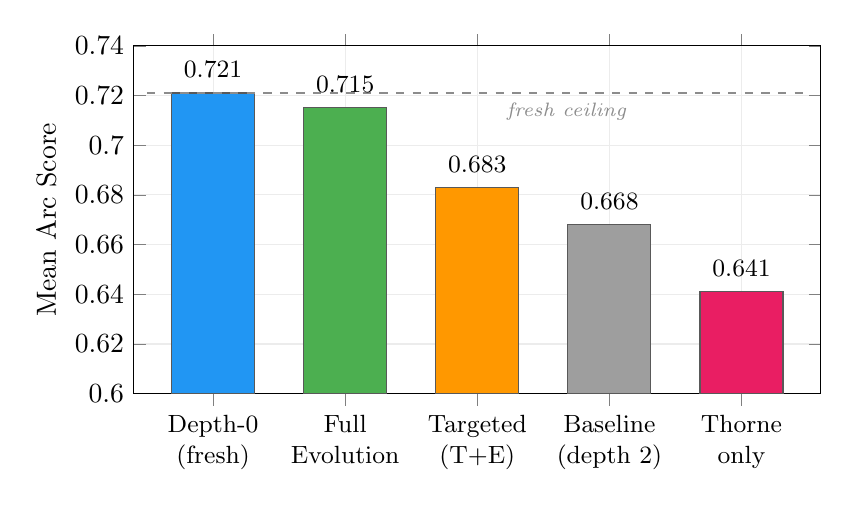
\begin{tikzpicture}
\begin{axis}[
  width=0.85\textwidth,
  height=6cm,
  ybar,
  bar width=30pt,
  bar shift=0pt,
  ylabel={Mean Arc Score},
  ymin=0.60, ymax=0.74,
  xmin=-0.6, xmax=4.6,
  ytick={0.60,0.62,0.64,0.66,0.68,0.70,0.72,0.74},
  xtick={0,1,2,3,4},
  xticklabels={Depth-0\\(fresh),Full\\Evolution,Targeted\\(T+E),Baseline\\(depth 2),Thorne\\only},
  x tick label style={font=\small, align=center},
  nodes near coords,
  nodes near coords style={font=\small, above, yshift=2pt},
  every node near coord/.append style={/pgf/number format/.cd, fixed, fixed zerofill, precision=3},
  grid=major,
  grid style={gray!15},
  enlarge x limits=false,
  clip=false,
]
\addplot[draw=black!65, fill=cfresh]    coordinates {(0,0.721)};
\addplot[draw=black!65, fill=cfull]     coordinates {(1,0.715)};
\addplot[draw=black!65, fill=ctargeted] coordinates {(2,0.683)};
\addplot[draw=black!65, fill=cbaseline] coordinates {(3,0.668)};
\addplot[draw=black!65, fill=cthorne]   coordinates {(4,0.641)};
% Depth-0 reference line
\draw[dashed, black!45, semithick] (axis cs:-0.5,0.721) -- (axis cs:4.5,0.721);
\node[font=\scriptsize\itshape, text=black!45, anchor=north west] at (axis cs:2.15,0.721) {fresh ceiling};
\end{axis}
\end{tikzpicture}
\caption{Mean arc quality scores across five experimental conditions. Dashed line marks the depth-0 (fresh) ceiling. Full evolution closes 89\% of the gap between baseline and fresh. Thorne-only evolution \emph{degrades} quality below baseline, revealing a collective threshold effect.}
\label{fig:score_comparison}
\end{figure*}

\begin{table}[t]
\centering
\caption{Arc quality across conditions. Full evolution closes 89\% of the gap between baseline and fresh simulations. Means are over valid arcs only.}
\label{tab:conditions}
\begin{tabular}{lccc}
\toprule
\textbf{Condition} & \textbf{Mean} & \textbf{$\Delta$ Base} & \textbf{$\Delta$ Fresh} \\
\midrule
Depth-0 (fresh)      & 0.721 & $+$0.053 & --- \\
Full evolution        & 0.715 & $+$0.047 & $-$0.006 \\
Targeted (T+E)       & 0.683 & $+$0.015 & $-$0.038 \\
Baseline (depth~2)   & 0.668 & ---      & $-$0.053 \\
Thorne-only$^\dag$   & 0.641 & $-$0.027 & $-$0.080 \\
\bottomrule
\multicolumn{4}{@{}l}{\footnotesize $^\dag$\,5/6 valid arcs (Marcus arc invalid).}
\end{tabular}
\end{table}

Figure~\ref{fig:score_comparison} and Table~\ref{tab:conditions} present aggregate scores. Full evolution achieves a mean of 0.715, closing 89\% of the 0.053-point gap between baseline (0.668) and fresh (0.721). The relationship between agent count and quality is non-monotonic: evolving one agent degrades quality below baseline ($-0.027$), two agents partially recover ($+0.015$), and six agents approach the fresh ceiling ($+0.047$). This collective threshold pattern---partial evolution is counterproductive, while comprehensive evolution restores quality---is the central empirical finding of this paper.

\begin{table*}[t]
\centering
\caption{Per-agent arc scores across conditions. Elena shows the largest improvement under full evolution ($+0.258$ vs.\ baseline); Marcus shows the largest decline ($-0.067$). ``---'' indicates an invalid arc (excluded from condition means).}
\label{tab:per_agent}
\begin{tabular}{lcccccc}
\toprule
\textbf{Condition} & \textbf{Thorne} & \textbf{Elena} & \textbf{Marcus} & \textbf{Lydia} & \textbf{Diana} & \textbf{Victor} \\
\midrule
Depth-0 (fresh)      & 0.727 & 0.718 & 0.735 & 0.718 & 0.713 & 0.716 \\
Full evolution        & 0.718 & 0.726 & 0.656 & 0.728 & 0.743 & 0.720 \\
Targeted (T+E)       & 0.676 & 0.728 & 0.665 & 0.679 & 0.678 & 0.672 \\
Baseline (depth~2)   & 0.709 & 0.468 & 0.723 & 0.719 & 0.706 & 0.685 \\
Thorne-only          & 0.663 & 0.614 & ---   & 0.665 & 0.626 & 0.639 \\
\bottomrule
\end{tabular}
\end{table*}

\begin{table}[t]
\centering
\caption{Event type distribution (reported types; T-only = Thorne-only evolution). Full evolution shifts the genre profile: conflict and catastrophe increase while chat and physical decrease.}
\label{tab:events}
{\small
\begin{tabular}{@{}lrrrrr@{}}
\toprule
\textbf{Type} & \textbf{D-0} & \textbf{Base} & \textbf{T+E} & \textbf{Full} & \textbf{T-only} \\
\midrule
chat        & 21 & 24 & 21 & 13 & 20 \\
conflict    & 7  & 7  & 9  & 13 & 9  \\
reveal      & 6  & 2  & 4  & 0  & 3  \\
lie         & 6  & 6  & 5  & 5  & 4  \\
confide     & 10 & 4  & 1  & 4  & 0  \\
catastrophe & 3  & 2  & 7  & 7  & 4  \\
physical    & 16 & 20 & 13 & 11 & 11 \\
observe     & 42 & 43 & 76 & 59 & 66 \\
\bottomrule
\end{tabular}
}
\end{table}

Table~\ref{tab:per_agent} shows per-agent breakdowns. Table~\ref{tab:events} reveals the mechanism: full evolution nearly doubles \textsc{conflict} events ($7 \to 13$) and more than triples \textsc{catastrophe} events ($2 \to 7$), while reducing low-tension \textsc{chat} ($24 \to 13$) and routine \textsc{physical} ($20 \to 11$). The baseline's suppressed \textsc{reveal} count (2 vs.\ 6 in fresh) reflects the information depletion problem directly: with most secrets already known, there is nothing left to reveal.

\subsection{Key Findings}

\paragraph{Finding 1: Elena as canary.}
Elena's baseline arc score (0.468) is a dramatic outlier---the only agent below 0.60. Her original goal structure (secrecy~0.90, commitment to maintain secrecy) produces incoherent behavior when the affair is universally known (Table~\ref{tab:canon_state}). Full evolution restores her to 0.726 ($+0.258$), the largest single-agent improvement, by replacing secrecy-oriented goals with post-revelation motivations.

\smallskip
\paragraph{Finding 2: Collective threshold.}
Evolving Thorne alone \emph{degrades} mean quality by $-0.027$ and invalidates Marcus's arc entirely (5/6 valid). Evolving Thorne and Elena together recovers only $+0.015$. Full six-agent evolution achieves $+0.047$. This non-monotonic pattern suggests a coordination requirement: partial evolution is counterproductive, while comprehensive evolution achieves near-complete recovery. Locating the precise threshold requires 3-, 4-, and 5-agent conditions (future work). The finding supports the hypothesis that, in our system, narrative quality is strongly shaped by the agent interaction topology: Thorne's evolved hostility toward Marcus produces good narrative structure only when Marcus, Lydia, Diana, and Victor have adapted their goals to respond coherently.

\begin{table*}[t]
\centering
\caption{Wound topology across conditions. \ding{51} indicates wound pattern present; ``---'' indicates absent. Population frequency (Pop.~Freq.) is the fraction of 50 baseline seeds exhibiting each pattern. Full evolution restructures the conflict graph, losing 3 wounds and gaining 2.}
\label{tab:wounds}
{\small
\begin{tabular}{lccccccc}
\toprule
\textbf{Wound Pattern} & \textbf{Pop.\ Freq.} & \textbf{Depth-0} & \textbf{Baseline} & \textbf{Targeted} & \textbf{Full} & \textbf{Thorne-only} \\
\midrule
Marcus--Victor   & 0.94 & \ding{51} & \ding{51} & \ding{51} & \ding{51} & \ding{51} \\
Diana--Thorne    & 0.90 & \ding{51} & ---           & \ding{51} & \ding{51} & \ding{51} \\
Thorne--Victor   & 0.90 & \ding{51} & \ding{51} & \ding{51} & ---           & \ding{51} \\
Elena--Thorne    & 0.86 & \ding{51} & \ding{51} & \ding{51} & \ding{51} & ---           \\
Lydia--Marcus    & 0.78 & \ding{51} & \ding{51} & \ding{51} & ---           & \ding{51} \\
Lydia--Thorne    & 0.66 & ---           & \ding{51} & \ding{51} & ---           & \ding{51} \\
Marcus--Thorne   & 0.56 & \ding{51} & ---           & \ding{51} & \ding{51} & \ding{51} \\
Diana--Victor    & 0.50 & ---           & \ding{51} & ---           & \ding{51} & ---           \\
\midrule
\textbf{Total}   &      & \textbf{6}   & \textbf{6}   & \textbf{7}   & \textbf{5}   & \textbf{6} \\
\bottomrule
\end{tabular}
}
\end{table*}

\smallskip
\paragraph{Finding 3: Wound topology restructuring.}
Table~\ref{tab:wounds} shows the full wound topology across conditions. Full evolution causes three wound patterns to disappear (Thorne--Victor, Lydia--Marcus, Lydia--Thorne) and two to appear (Diana--Thorne, Marcus--Thorne), producing a net reduction from 6 to 5 active wounds. The persistent wound Marcus--Victor (population frequency 0.94) survives all conditions, suggesting it reflects a structural property of the scenario rather than a belief-contingent pattern.

\smallskip
\paragraph{Finding 4: Overlap redistribution.}
Baseline arcs show high pairwise overlap (top Jaccard: 0.481, Lydia--Thorne), indicating convergence toward similar events. Full evolution reduces maximum overlap to 0.379, producing more narratively distinct per-protagonist arcs---the different agents' stories diverge more under coordinated evolution.

\smallskip
\paragraph{Finding 5: Immediate divergence.}
All evolution conditions diverge from baseline at tick~0---the first decision cycle. Because goal vectors are direct inputs to $u_{\text{base}}$ (Eq.~\ref{eq:utility}), any goal change immediately alters action selection. This contrasts with the perturbation experiment's control mutation, which produced zero divergence.


% ============================================================
% 7. DISCUSSION
% ============================================================
\section{Discussion}
\label{sec:discussion}

\subsection{Information Equilibrium}

Chain degradation can be understood through an information-theoretic lens. A fresh simulation begins with high \emph{dramatic potential}: secrets are unknown, relationships are ambiguous, and the space of information-revealing actions is large. As episodes accumulate and secrets resolve, the system approaches an information equilibrium. The canon state in Table~\ref{tab:canon_state} makes this concrete: after just two episodes, 24 of 42 agent-claim pairs (57\%) are \texttt{believes\_true}, and four of five secret claims are universally known. The decision engine still reads these beliefs every tick (13{,}895 reads in our traced run), but they no longer create utility gradients that differentiate between actions.

Goal evolution operates as a \emph{gradient injection} mechanism: by changing what agents value, it creates new utility gradients without requiring new secrets or propositions. Thorne shifting from loyalty-oriented to truth-seeking goals makes previously low-utility actions (confrontation, investigation) newly attractive, restoring the conditions for dramatic arc formation.

\subsection{Collective Threshold}

The non-monotonic relationship between evolved agent count and quality recovery suggests a collective threshold phenomenon in our system. One evolved agent in a system of five unevolved agents produces \emph{worse} outcomes than no evolution, because the evolved agent's new behavior is met with response patterns calibrated for the old interaction dynamics. Two evolved agents achieve partial recovery. Six achieve near-complete recovery. The pattern suggests that a substantial fraction of the interaction graph must be updated for coherent collective behavior to emerge; pinpointing the precise threshold between 2 and 6 agents requires additional intermediate conditions (3, 4, and 5 evolved agents) left for future work. Whether this coordination requirement generalizes beyond our six-agent scenario is an open question.

\subsection{Implications for Serial Narrative}

These results have practical implications for systems generating season-length narrative content. Rather than accumulating secrets and resolutions that gradually deplete dramatic potential, such systems could implement periodic goal evolution passes---analogous to character development between seasons of a television series---where agent motivations are updated to reflect the narrative consequences of prior episodes. The 89\% quality recovery demonstrated here suggests that goal evolution alone, without introducing new characters, locations, or secrets, may be sufficient to sustain narrative quality across longer episode sequences than fixed-goal baselines can support.

\subsection{On Hand-Tuned Evolution}

A natural objection is that hand-tuned goal evolution simply encodes good character development by authorial fiat. However, the critical finding is not that particular goal values produce quality recovery, but that the \emph{topology} of evolution matters: identical evolution style applied to one agent degrades quality and invalidates a co-protagonist's arc, while the same style applied across all agents achieves near-complete recovery. This coordination requirement is not an artifact of the specific mutation values---it reflects a structural property of how multi-agent utility landscapes interact. Automated goal evolution (Section~\ref{sec:future}) would test whether machine-generated mutations exhibit the same coordination requirement.

\subsection{Limitations}

\begin{enumerate}[nosep]
\item \textbf{Single scenario.} All experiments use the Dinner Party scenario with six agents and five locations. Generalization to larger populations, different social dynamics, or non-social scenarios remains untested.
\item \textbf{Hand-tuned mutations.} Goal evolution profiles were manually designed to reflect plausible character development. Automated goal evolution is future work.
\item \textbf{Single seed per condition.} The Rashomon sweep validates baseline quality across 50 seeds ($\sigma = 0.037$), but the goal evolution experiment uses seed~7 only. Seed-specific interactions between initial conditions and goal mutations cannot be ruled out.
\item \textbf{Composite scoring.} Arc quality is a weighted composite of seven dimensions (Eq.~\ref{eq:composite}). Different weightings could change condition rankings, though tension-related and non-tension dimensions are balanced at 50/50.
\item \textbf{Depth-2 chain.} We test at canon depth~2. Deeper chains may require more aggressive evolution or additional mechanisms.
\item \textbf{No human evaluation.} All quality judgments are automated metrics; perceptual quality of narrated output has not been assessed.
\end{enumerate}


% ============================================================
% 8. FUTURE WORK
% ============================================================
\section{Future Work}
\label{sec:future}

\paragraph{Stance machines.} Hand-tuned evolution profiles could be replaced by pre-defined goal archetypes---\emph{stance profiles}---with deterministic transitions (e.g., Elena.\textsc{the\_concealer}~$\to$ Elena.\textsc{the\_survivor}). Selection between stances at episode boundaries could use constrained classifiers conditioned on prior-episode metrics, providing structured goal evolution without per-field tuning.

\paragraph{Structural gradient ascent.} At \$0.00 per deterministic run, brute-force sensitivity sweeps over the goal vector space are computationally feasible. Systematic evaluation of goal mutations by their downstream arc quality impact could identify optimal evolution configurations without hand-tuning.

\paragraph{Affordance injection.} Goal evolution restores quality by creating new utility gradients over \emph{existing} information. Complementarily, introducing new information objects---evidence, leverage, commitments---at episode boundaries would provide fresh dramatic fuel alongside evolved goals.

\paragraph{Alternative scenarios.} The Dinner Party relies on information asymmetry (secrets, social alliances) as its primary dramatic fuel. Whether chain degradation occurs in exploration or quest scenarios---where dramatic potential derives from spatial discovery rather than social revelation---remains an open question that would test generality of the information depletion mechanism.

\paragraph{Scaling experiments.} Testing with larger agent populations, deeper chains (5--10 episodes), and multiple scenario types would establish the generality of the degradation and collective-threshold phenomena.

\paragraph{Human evaluation.} A perceptual quality study comparing narrated output from baseline versus evolved conditions would validate whether the automated arc score improvements correspond to human judgments of narrative quality.


% ============================================================
% 9. CONCLUSION
% ============================================================
\section{Conclusion}
\label{sec:conclusion}

We have demonstrated that multi-episode narrative simulations with persistent world state face a systematic chain degradation problem rooted in goal--world misalignment. Through controlled perturbation experiments, we provided evidence that, within our deterministic pipeline, belief-state content causally affects narrative structure, with structurally central propositions producing order-of-magnitude larger effects than peripheral controls. Coordinated goal evolution across all agents closes 89\% of the quality gap, approaching fresh-simulation quality without discarding accumulated canon. The collective nature of this recovery---single-agent evolution degrades quality while coordinated evolution restores it---suggests that narrative quality in multi-agent simulation is strongly shaped by the interaction topology rather than by individual character properties alone.

These findings suggest that the longstanding challenge of maintaining narrative quality in extended multi-agent simulations may be addressable through principled goal adaptation mechanisms, opening a path toward simulation-driven serial narrative systems that sustain dramatic quality across longer episode sequences than fixed-goal baselines can support.

\bibliographystyle{plainnat}
\bibliography{references}

\end{document}
